\documentclass[10pt,twocolumn,letterpaper]{article}
\usepackage[margin=0.9in]{geometry}
\usepackage{graphicx}
\usepackage{amsmath,amssymb}
\usepackage{booktabs}
\usepackage{xcolor}
\usepackage[colorlinks=true,allcolors=blue]{hyperref}
\usepackage{caption}
\graphicspath{{figs/}}
\renewcommand{\ttdefault}{cmtt}

\title{Auditing Disocclusion Reliability Evidence:\ Diagnostic Separability Does Not Imply Observable Routing}
\author{Anonymous submission\\\small Paper ID ****}
\date{}

\begin{document}
\maketitle

\begin{abstract}
We audit whether a slow generative teacher's usefulness in single-view 3D
reconstruction can be predicted from inference-time evidence. The previously
reported frame result---ROC-AUC 0.947, trapezoidal PR-AUC 0.961, and
$+1.604$ dB at 41\% calls saved---uses ground-truth-derived PSNR quality probes.
It is a diagnostic, not deployment performance. On the same 2,898 frames and 74
scene-grouped folds, camera translation and rotation yield accuracy 0.612,
ROC-AUC 0.650, trapezoidal PR-AUC 0.663, and $+0.715$ dB, retain a $-23.094$ dB
worst case, and make 2,028 calls. E-223 combines RGB disagreement with
\texttt{visibility.npy}, which VGGT derives from the complete target clip; it is
therefore an oracle-visibility diagnostic. On a selected population of 910
frames from 21 high-gain scenes (96.5\% positive), it reaches ROC-AUC 0.426,
average precision 0.929, and calls every frame at threshold 0.5. Thus the release
supports diagnostic separability but no operational routing claim.
\end{abstract}

\section{Introduction}
A generative prior can improve disoccluded regions in feed-forward novel-view
reconstruction~\cite{flash3d} but can also cause severe losses. Reliability prediction would be useful only if its inputs exist before
GT and teacher evaluation. We revisit the evidence under this requirement and
separate four tiers: (i) oracle true gain, (ii) GT-quality-probe diagnostic,
(iii) camera-only observable evidence, and (iv) RGB disagreement +
oracle-visibility diagnostic evidence.

\paragraph{Contributions.}
\begin{enumerate}
\item We correct the provenance and semantics of the released frame features,
including the historical \texttt{vis\_gap} field.
\item We reproduce the full-population camera-only grouped-CV baseline and
contrast it with the quality-probe diagnostic upper bound.
\item We report the RGB-disagreement result as a selected-population negative
result and add executable feature-whitelist and claim-integrity checks.
\end{enumerate}

\section{Evidence Audit}
\begin{figure*}[t]
\centering
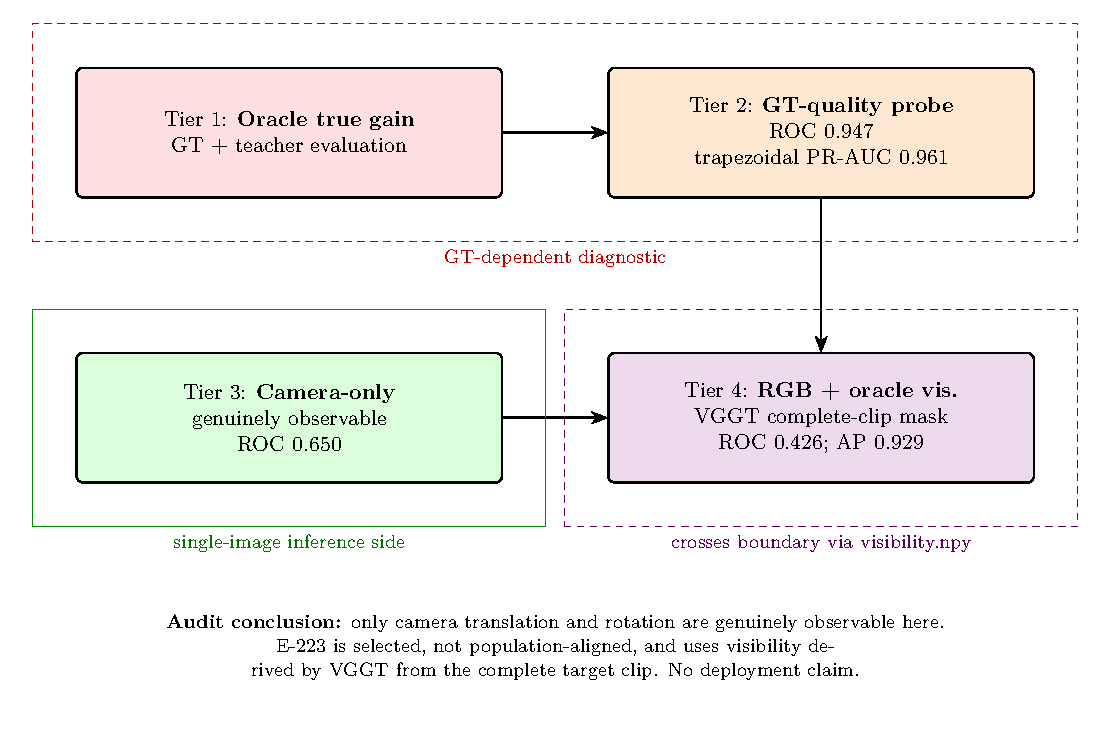
\includegraphics[width=0.9\textwidth]{fig_pipeline.pdf}
\caption{Four evidence tiers. Oracle true gain and GT-quality probes are
GT-dependent diagnostics. E-223 also crosses the boundary because VGGT derives
its visibility mask from the complete target clip. Only E-224 camera translation
and rotation are genuinely observable. No deployment claim is made.}
\label{fig:pipeline}
\end{figure*}

\paragraph{Labels and oracle.}
For frame $i$, gain is the teacher's invisible-region PSNR minus the baseline's
invisible-region PSNR, both evaluated against GT. The binary label is one when
gain exceeds 0.1 dB. Oracle decisions use true gain and are upper bounds.

\paragraph{Corrected feature semantics.}
The frame JSON is preserved, but its column names require care.
\texttt{f3d\_vis} and \texttt{f3d\_inv} are PSNR quality probes computed against
GT. Historical \texttt{vis\_gap} equals \texttt{f3d\_vis - base\_inv}; it is not
an expert-visible minus baseline-visible difference. Interactions built from
these columns remain GT-derived. Camera translation and rotation are observable.

\paragraph{Evaluation.}
All frame experiments use grouped leave-one-scene-out cross-validation: every
frame from the held-out scene is excluded from fitting. The camera-only and
quality-probe frame experiments share 2,898 frames and 74 scenes. The RGB
experiment instead uses 910 frames from 21 selected high-gain scenes, so it is
reported separately rather than as a controlled comparison.

\section{Results}
\begin{table*}[t]
\centering\small
\caption{Four evidence tiers. The first three rows share the 2,898-frame
population; E-223 uses 910 frames from 21 selected scenes. Precision-recall
metrics are labeled per row because E-223 reports average precision whereas
E-145b/E-224 use trapezoidal integration.}
\resizebox{\textwidth}{!}{%
\begin{tabular}{lllrrrl}
\toprule
Tier & Population & Predictor inputs & Acc. & ROC & Precision-recall & Mean / policy \\
\midrule
Oracle true gain & 2,898 / 74 scenes & True gain & -- & -- & -- & $+1.70$ dB upper bound \\
GT-quality-probe diagnostic & 2,898 / 74 scenes & GT PSNR probes + camera & 0.861 & 0.947 & Trap. PR-AUC 0.961 & $+1.604$ dB; 41\% saved \\
Camera-only observable & 2,898 / 74 scenes & Translation + rotation & 0.612 & 0.650 & Trap. PR-AUC 0.663 & $+0.715$ dB; 2,028 calls \\
RGB + oracle-vis. diagnostic & 910 / 21 selected & RGB + VGGT visibility + camera & 0.965 & 0.426 & Average precision 0.929 & all 910 called \\
\bottomrule
\end{tabular}%
}
\label{tab:audit}
\end{table*}

\subsection{Quality probes reveal diagnostic separability}
E-145b reaches ROC-AUC 0.947 and trapezoidal PR-AUC 0.961. Its threshold-0.5 policy obtains
$+1.604$ dB and skips 41\% of calls. These numbers show that frame outcomes have
strong structure when GT-derived reconstruction quality is supplied. They do not
measure inference-time prediction. The old frontier and routing strip are kept
only as diagnostic views of this upper bound.

\begin{figure*}[t]
\centering
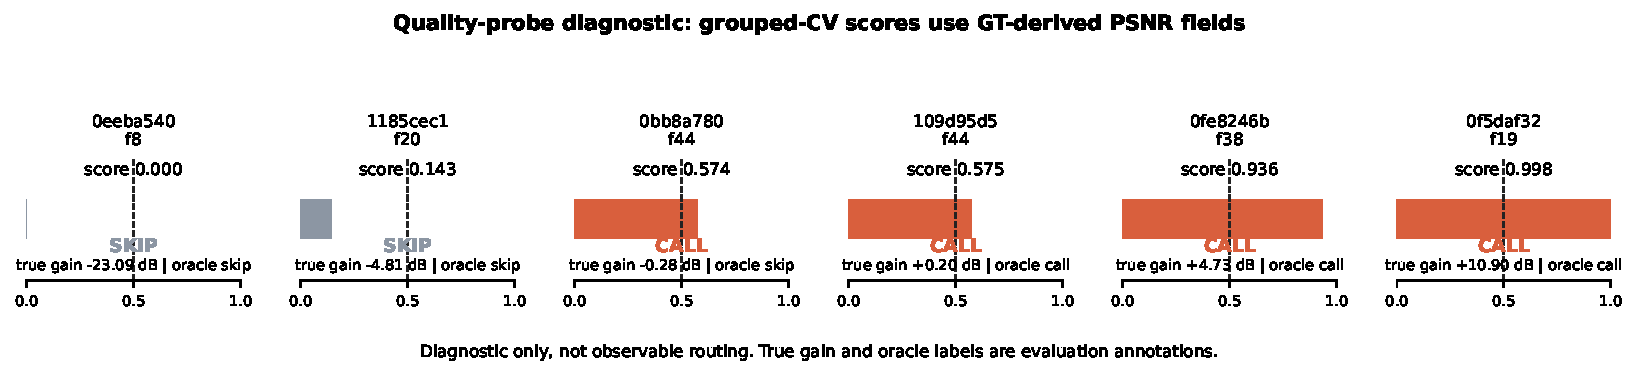
\includegraphics[width=\textwidth]{fig_routing_strip.pdf}
\caption{Quality-probe diagnostic strip from the released E-145b JSON inputs.
The grouped-CV scores depend on GT-derived PSNR probes. True gain and labels are
evaluation annotations. This illustrates diagnostic separability, not an
observable or operational routing process.}
\label{fig:routing}
\end{figure*}

\subsection{Observable camera evidence is insufficient}
E-224 admits exactly two predictors: target-camera translation and rotation
relative to the source. On all 2,898 frames it reaches accuracy 0.6118, ROC-AUC
0.6496, and trapezoidal PR-AUC 0.6631. At threshold 0.5 it calls 2,028 frames, saves 870
(30.0\%), and obtains $+0.7152$ dB mean gain. Its $-23.0944$ dB worst case is the
same severe loss exposed by always calling, so the result does not establish a
safe policy.

\subsection{RGB disagreement + oracle-visibility diagnostic}
E-223 uses baseline/Flash3D disagreement, image gradients, camera motion, and
\texttt{visibility.npy}. VGGT derives this mask from the complete target clip,
so it crosses the single-image inference boundary. Its 21 scenes are selected by
complete-asset availability in the high-gain \texttt{teacher\_npy} directory,
not population-aligned with E-145b/E-224; exact IDs and counts are released in a
manifest. Of 910 frames, 878 (96.5\%) are positive. ROC-AUC is 0.4255, average
precision is 0.9290, and the threshold-0.5 model calls all frames. The high
accuracy and average precision reflect prevalence, not useful ranking.

\begin{figure*}[t]
\centering
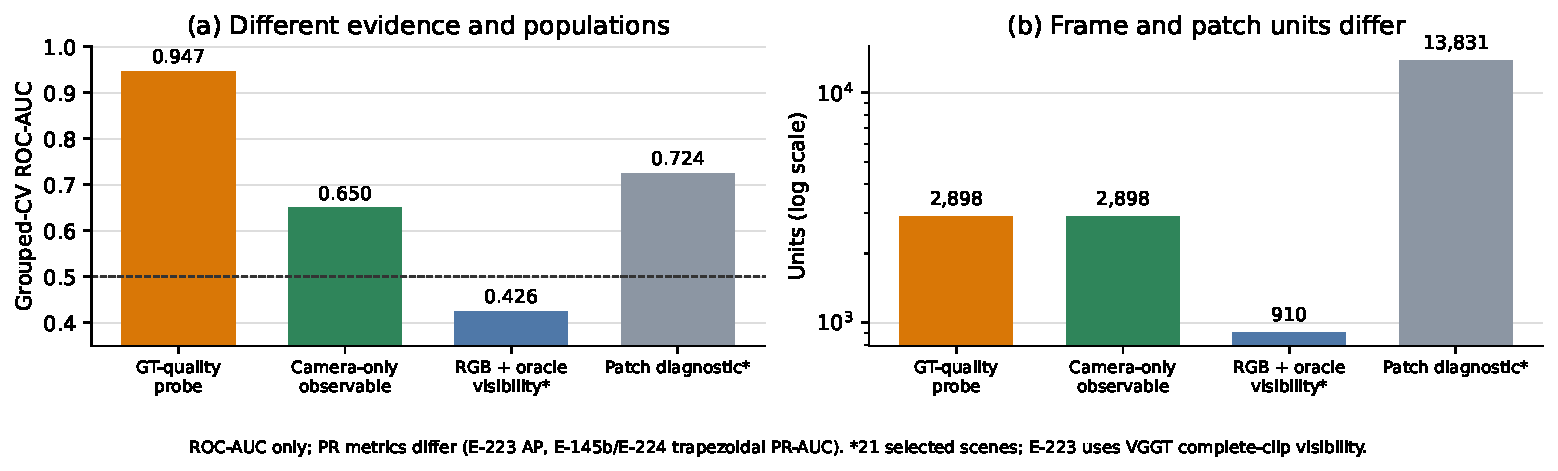
\includegraphics[width=\textwidth]{fig_granularity.pdf}
\caption{Diagnostic boundary, not a controlled leaderboard. Frame quality-probe
results use 2,898 frames from 74 scenes and report PSNR-based policy gain; patch
results use 13,831 patches from 21 selected high-gain scenes and patch-MSE-based
gain. Populations, units, prevalence, inputs, and gain metrics differ.}
\label{fig:granularity}
\end{figure*}

\section{Discussion}
The audit supports a narrower scientific result than the prior routing framing.
Teacher usefulness is highly separable at frame level with GT-derived quality
probes, which provides a useful target for future uncertainty estimators.
However, camera motion gives only modest full-population discrimination, while
E-223 fails to rank a heavily imbalanced selected set even with oracle visibility.
A valid operational claim requires stronger observable signals evaluated on the
same unselected population, followed by end-to-end latency and safety testing.

\section{Limitations}
E-223 and the patch study use selected high-gain scenes and cannot be directly
compared with the 74-scene frame population. E-223's rendered and VGGT visibility
assets are external, so only its aggregate and manifest are released. E-224 is
deliberately simple and does not rule out
better observable uncertainty features. The audit changes interpretation, not
released measurements.

\section{Conclusion}
GT-derived quality probes reveal strong frame-level diagnostic separability, but
this is not evidence of deployable routing. The full-population camera-only
baseline is substantially weaker, and the selected-population RGB + oracle-
visibility diagnostic is negative and limited. The evidence tiers and executable guards make that boundary
explicit.

{\small
\bibliographystyle{plain}
\bibliography{refs}
}
\end{document}
